\documentclass[10pt,landscape]{article}
\usepackage{multicol}
\usepackage{calc}
\usepackage{ifthen}
\usepackage[landscape]{geometry}
\usepackage{listings}
\usepackage{amsmath,amsthm,amsfonts,amssymb}
\usepackage{mathtools}
\usepackage{color,graphicx,overpic}
\usepackage{hyperref}
\usepackage[table, dvipsnames, xcdraw]{xcolor} % for \colorbox and named colors
\usepackage{transparent}

\usepackage{MnSymbol}
\usepackage{graphicx}
\usepackage{wrapfig}
\usepackage{tikz}

\usepackage{blindtext}

% This sets page margins to .1 inch if using letter paper, and to 1cm
% if using A4 paper. (This probably isn't strictly necessary.)
% If using another size paper, use default 1cm margins.
\ifthenelse{\lengthtest { \paperwidth = 11in}}
    { \geometry{top=0.2in,left=0.2in,right=0.2in,bottom=0.2in} }
    {\ifthenelse{ \lengthtest{ \paperwidth = 297mm}}
        {\geometry{top=1cm,left=1cm,right=1cm,bottom=1cm} }
        {\geometry{top=1cm,left=1cm,right=1cm,bottom=1cm} }
    }

% Turn off header and footer
\pagestyle{empty}

% Redefine section commands to use less space
\makeatletter
\renewcommand{\section}{\@startsection{section}{1}{0mm}%
                                {-1ex plus -.5ex minus -.2ex}%
                                {0.5ex plus .2ex}%x
                                {\normalfont\large\bfseries}}
\renewcommand{\subsection}{\@startsection{subsection}{2}{0mm}%
                                {-1ex plus -.5ex minus -.2ex}%
                                {0.5ex plus .2ex}%
                                {\normalfont\normalsize\bfseries}}
\renewcommand{\subsubsection}{\@startsection{subsubsection}{3}{0mm}%
                                {-1ex plus -.5ex minus -.2ex}%
                                {0.5ex plus .2ex}%
                                {\normalfont\footnotesize\bfseries}}
\makeatother

% Itemize to use less space
\usepackage{enumitem}
\setlist{leftmargin=*, nosep}
\setenumerate{nosep}

% Define BibTeX command
\def\BibTeX{{\rm B\kern-.05em{\sc i\kern-.025em b}\kern-.08em
    T\kern-.1667em\lower.7ex\hbox{E}\kern-.125emX}}

% Don't print section numbers
\setcounter{secnumdepth}{0}


\setlength{\parindent}{0pt}
\setlength{\parskip}{0pt plus 0.5ex}

%My Environments
\newtheorem{example}[section]{Example}

\newcommand{\Blue}[1]{\noindent{\textcolor{Blue}{\textbf{#1}}}:}
\newcommand{\Red}[1]{\noindent{\textcolor{BrickRed}{\textbf{#1}}}:}
\newcommand{\Green}[1]{\noindent{\textcolor{PineGreen}{\textbf{#1}}}:}
\newcommand{\Hint}[1]{\noindent{\textcolor{Orange}{#1}}}

\newcommand{\TODO}[1]{%
  \vspace{1em}%
  \noindent\textbf{\Large\textcolor{BrickRed}{TODO: #1}}%
  \vspace{1em}%
}

\newcommand*{\eg}{e.g.\@\xspace}
\newcommand*{\ie}{i.e.\@\xspace}
\newcommand*{\Eg}{E.g.\@\xspace}
\newcommand*{\Ie}{I.e.\@\xspace}
\newcommand*{\esp}{esp.\@\xspace}
\newcommand*{\wrt}{\ifmmode \stext{w.r.t.} \else w.r.t.\@\xspace \fi}


\usepackage{draftwatermark}
% Configure the watermark
\SetWatermarkText{Made with love by \texttt{junruren}} % Set the watermark text
\SetWatermarkScale{0.35}            % Adjust the scale of the watermark
\SetWatermarkLightness{0.9}      % Set the lightness (closer to 1 is more faded)
% -----------------------------------------------------------------------

\begin{document}
\raggedright
\scriptsize

\begin{multicols}{4}
% multicol parameters
% These lengths are set only within the two main columns
%\setlength{\columnseprule}{0.25pt}
\setlength{\premulticols}{1pt}
\setlength{\postmulticols}{1pt}
\setlength{\multicolsep}{1pt}
\setlength{\columnsep}{2pt}

\subsection{Diversification}

\subsubsection{Asset return characteristics}

Buy an asset (\eg a stock) at $t = 0$ at price $P_0$. At time $t = 1$,
\begin{itemize}
    \item its cash flow (dividend) is $D_1$, and
    \item its price is $P_1$
\end{itemize}
(both are random variables). The risk-free rate is $r_F$.

\Blue{Realized return}
\fbox{$r_1 = \frac{D_1 + P_1}{P_0} - 1$}
Returns comes from both dividends and capital gains.

\Blue{Expected return}
\fbox{$E[r_1] = \frac{E[D_1] + E[P_1]}{P_0} - 1$}

\Blue{Excess return} (realized)
\fbox{$r_1 - r_F$}

\Blue{Risk premium} (expected excess return) \fbox{$E[r_1] - r_F$}

\Red{Mean (average) return}
\fbox{$\bar{r} = E[r] = \frac{1}{T} \sum_{t=1}^T r_t$}
Would be same as the expected return $E[r_t]$ if expected returns are constant for all $t$.

\subsection{Options}

\Red{Options}
Derivative contracts specifying \textbf{a right} to \textbf{buy (call option)} or \textbf{sell (put option)} an underlying asset at a specified price $K$ (the \textbf{strike/exercise price}) on or before a specified date $T$ (the \textbf{expiration/maturity date}).

\begin{itemize}
    \item \Blue{Call option}: right to buy the underlying asset at the strike price.
    \item \Blue{Put option}: right to sell the underlying asset at the strike price.
\end{itemize}

Exercise style:
\begin{itemize}
    \item \Blue{American option}: can be exercised at any time before expiration.
    \item \Blue{European option}: can only be exercised at expiration.
\end{itemize}

\subsubsection{Option Payoff curves}

\begin{itemize}
    \item \Blue{$S$} Price of the underlying asset at expiration
    \item \Blue{$K$} Strike price of option
    \item \Hint{Payoff $\neq$ Profit}. To get profit (net payoff), need to subtract the option's cost.
\end{itemize}

\begin{multicols}{2}
\tiny \textbf{Payoff of buying a Call}
$\max(0, S - K)$
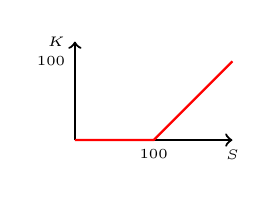
\begin{tikzpicture}
    % Draw lines
    \draw[->,thick] (0,0) -- (2,0) node[anchor=north] {\tiny $S$}; % Asset Price axis
    \draw[->,thick] (0,0) -- (0,1.25) node[anchor=east] {\tiny $K$}; % Strike Price axis
    % Draw payoff lines
    \draw[-,thick,red] (0,0) -- (1,0) -- (2,1);

    % Label values
    \node[anchor=north] at (1,0) {\tiny $100$};
    \node[anchor=east] at (0,1) {\tiny $100$};
\end{tikzpicture}

\tiny \textbf{Payoff of buying a Put}
$\max(0, K - S)$
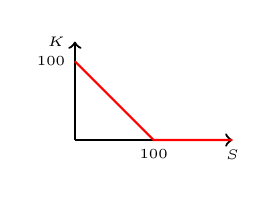
\begin{tikzpicture}
    % Draw lines
    \draw[->,thick] (0,0) -- (2,0) node[anchor=north] {\tiny $S$}; % Asset Price axis
    \draw[->,thick] (0,0) -- (0,1.25) node[anchor=east] {\tiny $K$}; % Strike Price axis
    % Draw payoff lines
    \draw[-,thick,red] (0,1) -- (1,0) -- (2,0);

    % Label values
    \node[anchor=north] at (1,0) {\tiny $100$};
    \node[anchor=east] at (0,1) {\tiny $100$};
\end{tikzpicture}

\tiny \textbf{Payoff of selling a Call}
$-\max(0, S - K)$
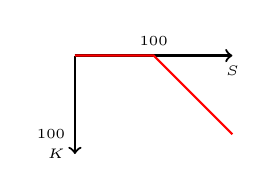
\begin{tikzpicture}
    % Draw lines
    \draw[->,thick] (0,0) -- (2,0) node[anchor=north] {\tiny $S$}; % Asset Price axis
    \draw[->,thick] (0,0) -- (0,-1.25) node[anchor=east] {\tiny $K$}; % Strike Price axis
    % Draw payoff lines
    \draw[-,thick,red] (0,0) -- (1,0) -- (2,-1);

    % Label values
    \node[anchor=south] at (1,0) {\tiny $100$};
    \node[anchor=east] at (0,-1) {\tiny $100$};
\end{tikzpicture}

\tiny \textbf{Payoff of selling a Put}
$-\max(0, K - S)$
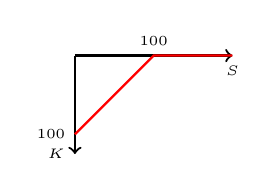
\begin{tikzpicture}
    % Draw lines
    \draw[->,thick] (0,0) -- (2,0) node[anchor=north] {\tiny $S$}; % Asset Price axis
    \draw[->,thick] (0,0) -- (0,-1.25) node[anchor=east] {\tiny $K$}; % Strike Price axis
    % Draw payoff lines
    \draw[-,thick,red] (0,-1) -- (1,0) -- (2,0);

    % Label values
    \node[anchor=south] at (1,0) {\tiny $100$};
    \node[anchor=east] at (0,-1) {\tiny $100$};
\end{tikzpicture}
\end{multicols}

Payoff curves of other assets that can be used with options:
\begin{multicols}{2}
\tiny Payoff of underlying asset
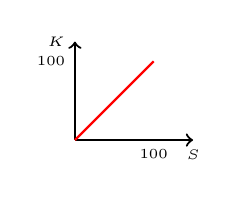
\begin{tikzpicture}
    % Draw lines
    \draw[->,thick] (0,0) -- (1.5,0) node[anchor=north] {\tiny $S$}; % Asset Price axis
    \draw[->,thick] (0,0) -- (0,1.25) node[anchor=east] {\tiny $K$}; % Strike Price axis
    % Draw payoff lines
    \draw[-,thick,red] (0,0) -- (1,1);

    % Label values
    \node[anchor=north] at (1,0) {\tiny $100$};
    \node[anchor=east] at (0,1) {\tiny $100$};
\end{tikzpicture}

\tiny Payoff of a \$100 FV ZC Bond
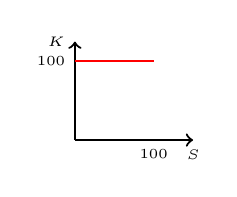
\begin{tikzpicture}
    % Draw lines
    \draw[->,thick] (0,0) -- (1.5,0) node[anchor=north] {\tiny $S$}; % Asset Price axis
    \draw[->,thick] (0,0) -- (0,1.25) node[anchor=east] {\tiny $K$}; % Strike Price axis
    % Draw payoff lines
    \draw[-,thick,red] (0,1) -- (1,1);

    % Label values
    \node[anchor=north] at (1,0) {\tiny $100$};
    \node[anchor=east] at (0,1) {\tiny $100$};
\end{tikzpicture}
\end{multicols}

\subsubsection{Option payoff and profit}

\begin{itemize}
    \item \Blue{$r$} Risk-free interest rate (EAR)
    \item \Blue{$C$} Call option price
    \item \Blue{$P$} Put option price
\end{itemize}

Call option:
\begin{tabular}{c|c|c|c}
    & $S < K$ & $S = K$ & $S > K$ \\
    \hline
    Payoff & $0$ & $0$ & $S - K$ \\
    Profit & $-C (1+r)^T$ & $-C (1+r)^T$ & $S - K - C (1+r)^T$ \\
\end{tabular}

Put option:
\begin{tabular}{c|c|c|c}
    & $S < K$ & $S = K$ & $S > K$ \\
    \hline
    Payoff & $K - S$ & $0$ & $0$ \\
    Profit & $K - S - P(1+r)^T$ & $- P(1+r)^T$ & $- P(1+r)^T$ \\
\end{tabular}

\end{multicols}
\end{document}